\paragraph{Tijdsduur}
\begin{figure}[H]
    \centering
    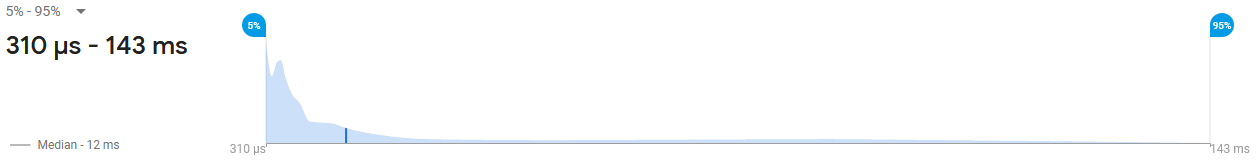
\includegraphics[height=0.1\textheight]{sensorenDuratieCrossAccelerometer.png}
    \caption{Overzicht tijdsduur ophalen van accelerometer data bij React Native.}
\end{figure}
Net zoals bij native worden er constant gegevens opgehaald vanaf dat de knop wordt ingedrukt om de
gegevens op te halen. Hierdoor worden er opnieuw honderden metingen gedaan die ons vertellen dat het ophalen
van de accelerometer data gemiddel 12ms duurt. De minimum en maximum waarden liggen op 310µs en 143ms.
Wat wel opvlat bij React Native is dat de eerste meting altijd langer duurt dan de rest. 
Hierdoor is het maximum veel hoger dan bij native. Bij native liggen de metingen dichter bij elkaar. 
\begin{figure}[H]
    \centering
    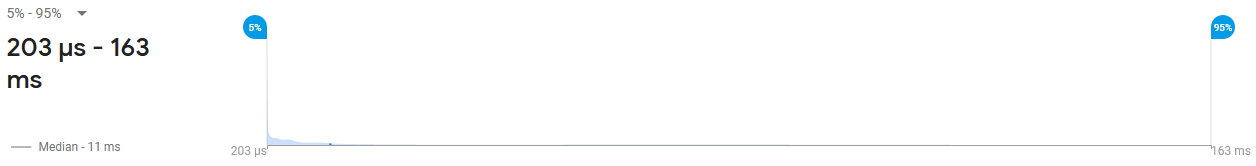
\includegraphics[height=0.1\textheight]{sensorenDuratieCrossGyroscoop.png}
    \caption{Overzicht tijdsduur ophalen van gyroscoop data bij React Native.}
\end{figure}
Net zoals bij de accelerometer worden er constant gegevens opgehaald vanaf dat de knop wordt ingedrukt om de 
gegevens op te halen. Hierdoor worden er opnieuw honderden metingen gedaan die ons vertellen dat het ophalen
van de gyroscoop data gemiddel 11ms duurt. De minimum en maximum waarden liggen op 203µs en 163ms.
Maar ook opnieuw zoals bij de accelerometer is de eerste meting veel trager dan de rest.

\paragraph{CPU \& geheugen}
\begin{figure}[H]
    \centering
    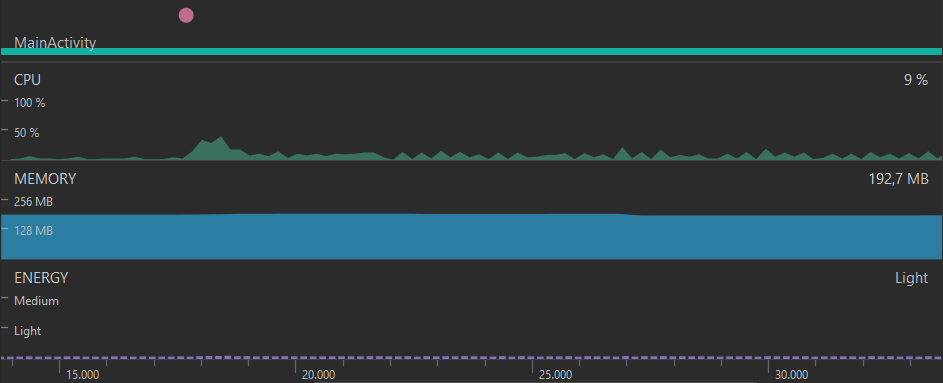
\includegraphics[height=0.25\textheight]{sensorenPerformantieCrossAccelerometer.png}
    \caption{Overzicht CPU en geheugen gebruik tijdens het ophalen van accelerometer data bij React Native.}
\end{figure}
Op de grafiek is te zien dat het CPU gebruik van de applicatie bij het ophalen van de accelerometer data,
piekt tot net geen 50\% en gemiddeld 9\% is na de piek. Wat opvalt is dat het CPU gebruik tijdens het ophalen 
van de data schommelt tussen 0\% en 20\%. Het geheugengebruik blijft stabiel rond de 192MB hangen, met verschillen van 
maximum 3-4MB. Ook is er opnieuw geen merkbaar verschil in het 
geheugen wanneer er data wordt opgehaald of wanneer er geen data wordt opgehaald.
\begin{figure}[H]
    \centering
    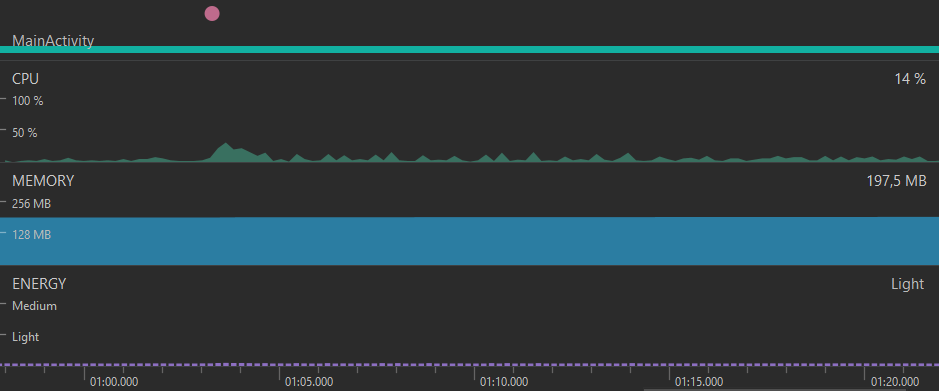
\includegraphics[height=0.25\textheight]{sensorenPerformantieCrossGyroscoop.png}
    \caption{Overzicht CPU en geheugen gebruik tijdens het ophalen van gyroscoop data bij React Native.}
\end{figure}
Net zoals bij native is er een piek in het CPU gebruik bij het starten van het ophalen van de gyroscoop data. 
De piek ligt hier wel hoger dan bij native, namelijk 40\%. Na de piek ligt het gemiddeld CPU gebruik ligt rond de 10\%. 
Net zoals bij de accelerometer schommelt het CPU gebruik tussen 0\% en 20\%. Het geheugen gebruik blijft terug 
stabiel rond de 197MB hangen, met verschillen van maximum 3-4MB. Net zoals bij de accelerometer is er  
geen merkbaar verschil in het geheugen wanneer er data wordt opgehaald of wanneer er geen 
data wordt opgehaald.
